\chapter{Introduction}
\section{Plan complexe}
On définit $\C\coloneqq\left\{a+b i\mid a,b\in\R\right\}$ où $i^2=-1$.$\C$ est un $\R-$espace vectoriel de dimension $2$ et de base $(1,i)$. Soit $z=a+bi$, on appelle $a$ la partie réel et $b$ la partie imaginaire.De ces notations/définitions on en crée une notation plus courante en Analyse.
\begin{definition}[Partie réel et Imaginaire]
    La partie réel d'un complexe $z$ est noté comme suit $\re(z)$ et on a 
    $$
    \re:\begin{cases}
        \C\longrightarrow\R\\
        a+bi\mapsto a
    \end{cases}$$
    et la partie imaginaire d'un complexe $z$ est noté comme suit $\im(z)$ et on a 
    $$
    \im:\begin{cases}
        \C\longrightarrow\R\\
        a+bi\mapsto b
    \end{cases}$$
\end{definition}
\begin{exemple}
    Soit $z=2-3i$. On a que $\re(z)=2$ et $\im(z)=-3$.
\end{exemple}

Comme $\C$ est un $\R-$espace vectoriel de dimension $2$, on le représente avec un plan avec en abscisse la partie réel et en ordonnée la partie imaginaire.

\begin{center}
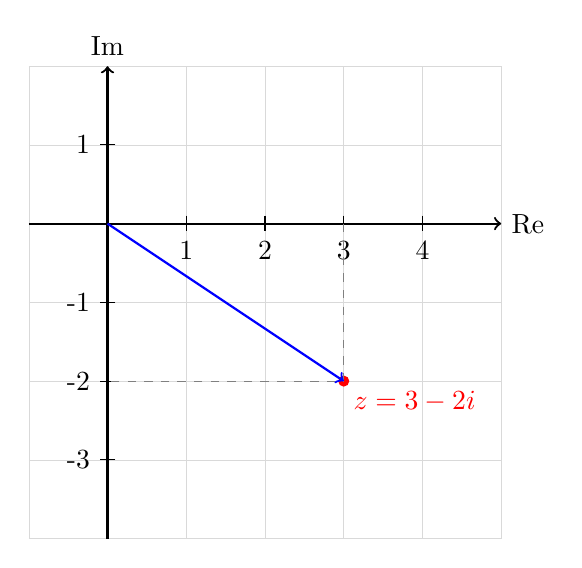
\begin{tikzpicture}
% Demo output for: Complex plane with z=3-2i plotted the angle showedgoing to 0 to arg(z)
     % Grille légère
    \draw[gray!30, very thin] (-1,-4) grid (5,2);

    % Axes
    \draw[->, thick] (-1,0) -- (5,0) node[right] {$\mathrm{Re}$};
    \draw[->, thick] (0,-4) -- (0,2) node[above] {$\mathrm{Im}$};

    % Graduations
    \foreach \x in {1,2,3,4}
        \draw (\x,0.1) -- (\x,-0.1) node[below] {\x};
    \foreach \y in {-3,-2,-1,1}
        \draw (0.1,\y) -- (-0.1,\y) node[left] {\y};

    % Point z = 3 - 2i
    \coordinate (z) at (3,-2);
    \fill[red] (z) circle (2pt);
    \node[below right, red] at (z) {$z = 3-2i$};

    % Projections pointillées
    \draw[dashed, gray] (3,0) -- (z) -- (0,-2);

    % Vecteur origine -> z
    \draw[->, blue, thick] (0,0) -- (z);
\end{tikzpicture}\\
\end{center}
\vspace{1cm}

\begin{definition}[Opération usuelles]
    Soient $z_1=a+bi$ et $z_2=c+di$ on définit alors $z_1+z_2=(a+c)+i(b+d)$ et $z_1z_2=(ac-bd)+i(ad+bc)$. On remarquera pour la 250 eme fois que ces opérations sont stables dans $\C$
\end{definition}
\begin{definition}[le module]
    Soit $z=a+bi$ on définit le module de $z$ noté $\abs{z}$ comme suit $$\abs{z}=\sqrt{a^2+b^2}$$
\end{definition}
\begin{remarque}[représentation des nombres complexes]
    Il existe majoritairement 3 formes de représentations de nombres complexes qui sont les suivantes:
    \begin{enumerate}
        \item Forme algébrique: $z=a+bi$
        \item Forme trigonométrique: $z=\abs{z}\cis(\theta)=\abs{z}\big(\cos(\theta)+ i\sin(\theta)\big)$
        \item Forme exponentielle: $z=\abs{z}\e^{i \theta}$
    \end{enumerate}
    où $\theta\in [0,2\pi]$ et $\theta\in[-\pi,\pi]$, on note généralement $\theta=\arg(z)$. On a que $\arg(0)$ n'est pas défini
\end{remarque}
\begin{remarque}[calcul de $\theta$]
    Notons que $\theta$ doit vérifier 
    $$\begin{cases}
        a=\abs{z}\cos(\theta)\\
        b=\abs{z}\sin(\theta)
    \end{cases}$$
\end{remarque}
La forme exponentielle a un intéret pour toutes les opérations d'ordre multiplicatif.
Soient $z=\abs{z}\e^{i\theta}$ et $z'=\abs{z'}\e^{i \theta'}$ Alors ;
\begin{enumerate}
    \item $zz'=\abs{z}\abs{z'}\e^{i(\theta+\theta')}=\abs{zz'}\e^{i(\theta+\theta')}=$
    \item $\forall n\in \Z, z^n=\abs{z}^n\e^{i n\theta}$
\end{enumerate}
Dans ce cours , on doit être capable de visualiser des ensembles 
\begin{exemple}
    Soient $A\coloneqq \left\{z\in\C\mid \abs{z-i}=1\right\}$ et $B\coloneqq \left\{z\in\C\mid \arg(z)=\frac{\pi}{2}\right\}$
\end{exemple}
\begin{center}
\begin{tikzpicture}[scale=1.2]
    
  % Quadrillage léger
  \draw[step=1cm, gray!25, thin] (-2.5,-1) grid (2.5,3.2);
  % Axes
  \draw[-{Stealth[length=2.5mm]}] (-2.5,0) -- (2.5,0) node[right] {$\mathrm{Re}(z)$};
  \draw[-{Stealth[length=2.5mm]}] (0,-1) -- (0,3.2) node[above] {$\mathrm{Im}(z)$};

  % Graduations
  \foreach \x in {-2,-1,1,2}
    \draw (\x,0.05) -- (\x,-0.05) node[below] {\scriptsize $\x$};
  \foreach \y in {1,2,3}
    \draw (0.05,\y) -- (-0.05,\y) node[left] {\scriptsize $\y$};

  % Ensemble A : cercle de centre i, rayon 1
  \draw[thick, blue] (0,1) circle (1);
  \fill[blue] (0,1) circle (1pt) node[below right] {\scriptsize $i$};
  \node[blue] at (1.6,1.6) {$A$};

  % Ensemble B : demi-droite arg(z) = pi/2 (axe imaginaire positif, sans l'origine)
  \draw[thick, red, -{Stealth[length=2.5mm]}] (0,0) -- (0,3);
  \node[red] at (0.5,2.7) {$B$};

  % Origine
  \fill (0,0) circle (0.8pt);
  \node[below left] {\scriptsize $0$};

  % Point d'intersection A ∩ B = {2i}
  \fill[violet] (0,2) circle (1.3pt);
  \node[violet, above right] at (0,2) {\scriptsize $2i$};

\end{tikzpicture}
\end{center}
Le fait de passer des réels aux complexes permet que toute équation de la forme $P(z)=0$ où $P$ est un polynôme non constant à coefficient dans $\C$ admet une solution dans $\C$ ($\C$ est algébriquement clos).
\section{Les fonctions de $\C$ dans $\C$}
Attention comme $\C$ est un $\R-$ espace vectoriel de dimension $2$, le graphe d'une fonction de $\C$ dans $\C$ vit dans un espace vectoriel de dimension $4$. Donc, on ne peut pas la visualiser.\\
Une chose que l'on peut faire , on peut visualiser $\re(f)$, $\im(f)$,$\abs{f}$,$\arg(f)$, \dots
\begin{exemple}
    Soit $f:\C\to\C$ tel que $\forall z=x+i y\in\C, f(z)=\bar{z}=x-i y$. On a $\forall z\in\C$ que \begin{enumerate}
        \item $\re(f(z))=\re(z)$
        \item $\im(f(z))=-\im(z)$
        \item $\abs{f(z)}=\abs{z}$
        \item $\arg(f(z))=-\arg(z)$
    \end{enumerate}
\end{exemple}
\begin{tikzpicture}[>=Stealth, every node/.style={font=\small}]

%%%%%%%%%%%%%%%%%%%%%%%%%%%%%%%%%%%%%%%%%%%%
% PLAN AVANT (gauche)
%%%%%%%%%%%%%%%%%%%%%%%%%%%%%%%%%%%%%%%%%%%%
\begin{scope}
  \draw[step=1cm, gray!20, thin] (-2.7,-2.7) grid (2.7,2.7);

  \draw[->] (-2.7,0) -- (2.7,0) node[right] {$\mathrm{Re}(z)$};
  \draw[->] (0,-2.7) -- (0,2.7) node[above] {$\mathrm{Im}(z)$};

  % Cercle unité, sens trigo (anti-horaire), plusieurs flèches
  \draw[thick, blue,
        decoration={markings,
          mark=at position 0.13 with {\arrow{latex}},
          mark=at position 0.38 with {\arrow{latex}},
          mark=at position 0.63 with {\arrow{latex}},
          mark=at position 0.88 with {\arrow{latex}}},
        postaction={decorate}]
    (0,0) circle (1);

  % Droite Re(z) = 1
  \draw[thick, red] (1,-2.7) -- (1,2.7);
  \node[red] at (1.6,2.3) {$\mathrm{Re}(z)=1$};

  % Coeur retourné, centré en (-1.6,-1.4)
  \draw[thick, violet, domain=0:360, samples=150, smooth, variable=\t]
    plot ({-1.6 + 0.055*16*sin(\t)^3},
          {-1.4 - 0.055*(13*cos(\t) - 5*cos(2*\t) - 2*cos(3*\t) - cos(4*\t))});
\end{scope}

%%%%%%%%%%%%%%%%%%%%%%%%%%%%%%%%%%%%%%%%%%%%
% FLECHE ARQUEE CENTRALE (style diagramme)
%%%%%%%%%%%%%%%%%%%%%%%%%%%%%%%%%%%%%%%%%%%%
\draw[->, thin] (3,2) to[bend left=35] node[midway, above=2pt] {$f$}
  node[midway, below=2pt] {\scriptsize $z\mapsto \bar z$} (5,2);

%%%%%%%%%%%%%%%%%%%%%%%%%%%%%%%%%%%%%%%%%%%%
% PLAN APRES (droite)
%%%%%%%%%%%%%%%%%%%%%%%%%%%%%%%%%%%%%%%%%%%%
\begin{scope}[xshift=8cm]
  \draw[step=1cm, gray!20, thin] (-2.7,-2.7) grid (2.7,2.7);

  \draw[->] (-2.7,0) -- (2.7,0) node[right] {$\mathrm{Re}(z)$};
  \draw[->] (0,-2.7) -- (0,2.7) node[above] {$\mathrm{Im}(z)$};
  % Cercle unité, sens horaire (orientation inversée), plusieurs flèches
  \draw[
    thick,
    blue,
    decoration={
        markings,
        mark=at position 0.13 with {\arrow{latex[reversed]}},
        mark=at position 0.38 with {\arrow{latex[reversed]}},
        mark=at position 0.63 with {\arrow{latex[reversed]}},
        mark=at position 0.88 with {\arrow{latex[reversed]}}
    },
    postaction={decorate}
] (0,0) circle (1);

  % Droite Re(z) = 1, invariante
  \draw[thick, red] (1,-2.7) -- (1,2.7);
  \node[red] at (1.6,2.3) {$\mathrm{Re}(z)=1$};

  % Coeur remis à l'endroit, centré en (-1.6,1.4)
  \draw[thick, violet, domain=0:360, samples=150, smooth, variable=\t]
    plot ({-1.6 + 0.055*16*sin(\t)^3},
          {1.4 + 0.055*(13*cos(\t) - 5*cos(2*\t) - 2*cos(3*\t) - cos(4*\t))});
  \node[violet] at (-1.6,2.3) {};
\end{scope}

\end{tikzpicture}
\begin{exemple}
    Soit $f:\C\to \C$. Soit $n\ge1$ ,un naturel, tel que $\forall z\in\C, f(z)=z^n$.On a que $\forall z\in \C$
    \begin{enumerate}
        \item $\abs{f(z)}=\abs{z}^n$
        \item $\arg(z^n)=n\arg(z)$
    \end{enumerate}
\end{exemple}
\begin{tikzpicture}[>=Stealth, every node/.style={font=\small}]

%%%%%%%%%%%%%%%%%%%%%%%%%%%%%%%%%%%%%%%%%%%%
% PLAN AVANT (gauche)
%%%%%%%%%%%%%%%%%%%%%%%%%%%%%%%%%%%%%%%%%%%%
\begin{scope}
  \draw[step=1cm, gray!20, thin] (-2.7,-2.7) grid (2.7,2.7);

  \draw[->] (-2.7,0) -- (2.7,0) node[right] {$\mathrm{Re}(z)$};
  \draw[->] (0,-2.7) -- (0,2.7) node[above] {$\mathrm{Im}(z)$};

  % Cercle unité, sens trigo (anti-horaire), plusieurs flèches
  \draw[thick, blue,
        decoration={markings,
          mark=at position 0.13 with {\arrow{latex}},
          mark=at position 0.38 with {\arrow{latex}},
          mark=at position 0.63 with {\arrow{latex}},
          mark=at position 0.88 with {\arrow{latex}}},
        postaction={decorate}]
    (0,0) circle (1);
\end{scope}

%%%%%%%%%%%%%%%%%%%%%%%%%%%%%%%%%%%%%%%%%%%%
% FLECHE ARQUEE CENTRALE (style diagramme)
%%%%%%%%%%%%%%%%%%%%%%%%%%%%%%%%%%%%%%%%%%%%
\draw[->, thin] (3,2) to[bend left=35] node[midway, above=2pt] {$f$}
  node[midway, below=2pt] {\scriptsize $z\mapsto z^n$} (5,2);

%%%%%%%%%%%%%%%%%%%%%%%%%%%%%%%%%%%%%%%%%%%%
% PLAN APRES (droite)
%%%%%%%%%%%%%%%%%%%%%%%%%%%%%%%%%%%%%%%%%%%%
\begin{scope}[xshift=8cm]
  \draw[step=1cm, gray!20, thin] (-2.7,-2.7) grid (2.7,2.7);

  \draw[->] (-2.7,0) -- (2.7,0) node[right] {$\mathrm{Re}(z)$};
  \draw[->] (0,-2.7) -- (0,2.7) node[above] {$\mathrm{Im}(z)$};
  % Cercle unité, sens horaire (orientation inversée), plusieurs flèches
  \draw[
    thick,
    blue,
    decoration={
        markings,
        mark=at position 0.13 with {\arrow{latex}},
        mark=at position 0.38 with {\arrow{latex}},
        mark=at position 0.63 with {\arrow{latex}},
        mark=at position 0.88 with {\arrow{latex}}
    },
    postaction={decorate}
] (0,0) circle (2.4);

\end{scope}

\end{tikzpicture}
\begin{exemple}
    Soit $f:\C\setminus\{0\}\to\C$ tel que $\forall z\in \C\setminus\{0\},f(z)=\frac{1}{z}$.
    On a que pour tout $z\in \C\setminus\{0\},$
    \begin{enumerate}
        \item $\re(f(z))=\frac{\re(z)}{\abs{z}^2}$
        \item $\im(f(z))=\frac{1}{\abs{z}}$
        \item $\abs{f(z)}=\frac{1}{\abs{z}}$
        \item $\arg(f(z))=-\arg(z)$
    \end{enumerate}
\end{exemple}
\begin{definition}[définition de l'exponentielle]
    On définit l'exponentielle complexe comme suit 
    $$\e^z:\begin{cases}
        \C\to\C\\
        z\mapsto\sum_{n\ge0}\frac{z^n}{n!}
    \end{cases}$$
    On remarque aisément via la théorie d'Analyse II que $z\mapsto\e^z$ est définie sur tout le plan complexe.De plus, on remarque trivialement qu'elle coincide avec l'exponentielle usuel sur les réels
\end{definition}
\begin{theoreme}[Formule d'Euler]
    On a l'égalité suivante 
    $$\forall t \in \R, \e^{i t}=\cos(t)+i \sin(t)$$
\end{theoreme}
\begin{proof}
    Soit $t\in \R$, montrons que $\e^{i t}=\cos(t)+i \sin(t)$\\
    Par la définition donnée précédemment, on a que 
    \begin{align*}
        \cos(t)+i\sin(t)&=\sum_{n=0}^{\infty}\frac{(-1)^nt^{2n}}{2n!}+i \sum_{n=0}^{\infty}\frac{(-1)^nt^{2n+1}}{(2n+1)!}\\
        &=\sum_{n\in2\N}\frac{i^nt^n}{n!}+i\sum_{n\in2\N+1}\frac{(i)^{n-1}t^n}{n!}\\
        &=\sum_{n\in\N}\frac{i^nt^n}{n!}=\sum_{n\in\N}\frac{(i t)^n}{n!}=\e^{i t}
    \end{align*}
\end{proof}
\begin{theoreme}
    $$\forall z_1,z_1\in\C, \e^{z_1+z_2}=\e^{z_1}\e^{z_2}$$
\end{theoreme}
\begin{proof}
    Soient $z_1,z_2\in \C,$ montrons que $\e^{z_1+z_2}=\e^{z_1}\e^{z_2}$. On a que $\forall n\in \N^{>0}$
    \begin{align*}
        \sum_{k=0}^{n}\frac{(z_1+z_2)^k}{k!}&=\sum_{k=0}^n\sum_{j=0}^k\frac{\binom{k}{j}z_1^jz_2^{k-j}}{k!}\\
        &=\sum_{k=0}^n\sum_{j=0}^k\frac{z_1^jz_2^{k-j}}{j!(k-j)!}\\
        &=\sum_{k=0}^n\sum_{p+q=k}\frac{z_1^pz_2^q}{p!q!}\\
        &=\sum_{p+q\le n}\frac{z_1^pz_2^q}{p!q!}\\
        &=\sum_{p=0}^n\frac{z_1^p}{p!}\sum_{q=0}^n\frac{z_2^q}{q!}-\sum_{n<p+q,p,q\le n}\frac{z_1^pz_2^q}{p!q!}
    \end{align*}
    On a que 
    \begin{equation*}
        \abs{\sum_{n<p+q,p,q\le n}\frac{z_1^pz_2^q}{p!q!}}\le\sum_{n<p+q,p,q\le n}\frac{\abs{z_1}^p\abs{z_2}^q}{p!q!}\le\sum_{k=n+1}^{2n}\frac{(\abs{z_1}+\abs{z_2})^k}{k!}
    \end{equation*}
    Comme $$\e^{\abs{z_1}+\abs{z_2}}=\sum_{k=0}^{\infty}\frac{(\abs{z_1}+\abs{z_2})^k}{k!}$$
    On a par le cours d'analyse II que $\lim_n\sum_{k=n+1}^{2n}\frac{(\abs{z_1}+\abs{z_2})^k}{k!}=0$. Donc finalement on trouve que 
    \begin{align*}
       \e^{z_1+z_2}&=\lim_n\sum_{k=0}^n \frac{(z_1+z_2)^k}{k!}\\
       &=\lim_n\Bigg(\sum_{p=0}^n\frac{z_1^p}{p!}\sum_{q=0}^n\frac{z_2^q}{q!}-\sum_{n<p+q,p,q\le n}\frac{z_1^pz_2^q}{p!q!}\Bigg)\\
       &=\e^{z_1}\e^{z_2}-0=\e^{z_1}\e^{z_2}
    \end{align*}
\end{proof}
Dès lors, on peut en conclure que $\forall z=x+i y, \e^z=\e^{x+i y}=\e^x\e^{i y}=\e^{x}(\cos(y)+i\sin(y))$
\begin{remarque}
    la fct $f(z)=\e^z$ est $2\pi i$ périodique
\end{remarque}
Dessin à mettre de la fct expo
\begin{definition}[Fonction trigonométrique]
    On définit les fonctions trigonométriques dans les complexes comme suit ;
    \begin{align*}
        &\sin(z)\coloneqq\frac{\e^{i z}-\e^{-i z}}{2i }=\sum_{n\ge0}\frac{(-1)^nz^{2n+1}}{(2n+1)!}\\
        &\cos(z)\coloneqq\frac{\e^{i z}+\e^{-i z}}{2}=\sum_{n\ge0}\frac{(-1)^nz^{2n}}{(2n)!}\\
    \end{align*}
    pour tout $z\in\C$
\end{definition}
\begin{definition}[fonction Logarithme]
    Comme la fonction exponentielle n'est pas une injection sur $\C$, il faut la restreindre à hauteur $2\pi$. On définit alors pour $y_0\in\R$
    $$A_{y_0}\coloneqq\{z=a+bi\mid y_0\le b\le y_0+2\pi\}$$
    On a ainsi que l'exponentielle est une injection de $A_{y_0}$ dans $\C\setminus\{0\}.$On a alors que la fonction reciproque de l'expo dans les complexe existe, souvent noté $\Ln(z)$. De plus, on a ;
    $$\Ln(z)=\ln(\abs{z})+i\arg_{y_0}(z)$$
    où $\arg_{y_0}(z)\in[y_0,y_0+2\pi[$.
\end{definition}
\begin{remarque}
    Le choix de $y_0$ a son importance.En effet, si $y_0=0$, on a que $\Ln(1)=1$. Si $y0=\pi$, alors $\Ln(1)=1+2i \pi$
\end{remarque}
\begin{remarque}
    Pour que $\Ln$ étende la fonction $\ln$ au complexe il faut choisir un $y_0$ dans $]-2\pi,0]$
\end{remarque}

Il manques des notes à partir d'ici faut les voler.

\section{Continuité pour les fonctions $f:\C\to\C$}

Comme $\C$ est muni du module $|\cdot |$, $( \C, |\cdot| )$ est un espace vectoriel normé.
\begin{definition}
    Soit $\Omega\subseteq U$. 
    \begin{itemize}
        \item $\Omega$ est ouvert si pour tout $z\in \Omega$, il existe $r>0$ tel que $$D(z,r) = \{\omega\in \C\mid \abs{\omega - z}<r\}\subseteq \Omega$$
        \item $\Omega$ est borné si il existe $R>0$ tel que $\Omega \subseteq D(0, R)$.
    \end{itemize}
\end{definition}

\begin{exemple}
    Pour illustrer :
    \begin{itemize}
        \item Le disque $D(z,r)$ est un ensemble ouvert et borné 
        \item $\C\setminus \{0\}$ est un ensemble ouvert qui n'est pas borné.
    \end{itemize}
\end{exemple}
\begin{definition}
    Soient $\Omega$ un ouvert et $f:\Omega \to \C$. Soit $z_0\in\Omega$. \begin{itemize}
        \item On dira que $f$ est continue en $z_0$ si $\lim_{z\to z_0}f(z) = f(z_0)$ ie $$\forall \varepsilon>0,\forall z \in \Omega, \abs{z-z_0}<\delta\alors \abs{f(z)-f(z_0)}$$
        \item On dira que $f$ est continu sur $\Omega$ si $f$ est continue en tout point de $\Omega$.
    \end{itemize}
\end{definition}
\begin{remarque}
Notons que :
    \begin{itemize}
        \item $\lim_{z\to z_0}f(z) = f(z_0)$ si et seulement si $\lim_{z\to z_0}\Re(f(z)) = \Re(f(z_0))$ et $\lim_{z\to z_0}\Im(f(z)) = \Im(f(z_0))$
        \item $f$ est continu sur $\Omega$ ssi $\Re(f), \Im(f)$ sont deux fonxtions continues sur $\R$.
    \end{itemize}
\end{remarque}
\begin{exemple}
    Toutes le fonctions vues précédemment sont continues sur leur domaine à l'exception du logarithme. En effet, si on considère $z_n = e^{i(y_0+2\pi - \frac{1}{n})}$ alors $z_n \to e^{i(y_0+2\pi)}= e^{iy_0}$ et $\ln(z_n)= \ln (|z_n|)+ i \operatorname{arg}(z_n)= i(y_0+2\pi - \frac{1}{n})\to i(y_0+2\pi)$ et pourtant $\ln(e^{iy_0})= iy_0$
\end{exemple}
Pour que $\Ln$ soit continu, il faut se restreindre à $\C$ privé de la demi-droite d'argument $y_0$. Notons que si on choisit $y_0= -\pi $, alors le logarithme est continu sur $\C \setminus \R ^-$.